% document
\documentclass[11pt, full]{article}
\usepackage[letterpaper, portrait, margin=0.75in]{geometry}
\usepackage{setspace}
\usepackage{color}

\RequirePackage{etoolbox}
\RequirePackage{pmboxdraw}
\RequirePackage[section]{minted}
\usemintedstyle{default}
\setminted[python]{linenos=false, frame=none}

\definecolor{bg}{rgb}{0.95, 0.95, 0.95}

\RequirePackage[many]{tcolorbox}
\tcbuselibrary{minted}

% text
\usepackage[utf8]{inputenc}
\setlength\parindent{0pt}
\setlength{\parskip}{1em}
\usepackage{enumitem}
\renewcommand{\familydefault}{\sfdefault}
\newcommand{\RomanNumeral}[1]{\textrm{\uppercase\expandafter{\romannumeral #1\relax}}}

\newcommand\yaq{\texttt{yaq}}

% math
\usepackage{amssymb}
\usepackage{amsmath}
\usepackage[cm]{sfmath}
\usepackage{commath}
\usepackage{multirow}
\DeclareMathAlphabet{\mathpzc}{OT1}{pzc}{m}{it}

% graphics
\usepackage{graphics}
\usepackage{graphicx}
\usepackage{epsfig}
\usepackage{epstopdf}
\usepackage{xpatch}
\graphicspath{{./figures/}}

% "S" prefix
\renewcommand{\theequation}{S\arabic{equation}}
\renewcommand{\thefigure}{S\arabic{figure}}
\renewcommand{\thetable}{S\arabic{table}}

% each section begins new page
\let\stdsection\section
\renewcommand\section{\clearpage\stdsection}

% force all floats to center (see https://tex.stackexchange.com/a/53383)
\makeatletter
\g@addto@macro\@floatboxreset{\centering}
\makeatother

% bibliography
\usepackage[backend=bibtex, natbib=true, url=false, sorting=none, maxbibnames=99]{biblatex}
\bibliography{references}

% hyperref
\usepackage[colorlinks=true, linkcolor=black, urlcolor=blue, citecolor=black, anchorcolor=black]
  {hyperref}
\usepackage[all]{hypcap}  % helps hyperref work properly


\NewTCBListing[number within=chapter, auto counter]{codefragment}{mo}{%
  %colback=bg,
  boxrule=1pt,
  %colframe=bg,
  arc=0pt,
  shadow=false,
  new/use counter=equation,
  boxsep=1ex, top=0pt, left=0pt, right=0pt, bottom=0pt,
  comment={\hfill(\arabic{chapter}.\arabic{equation})},
  listing outside comment,
  righthand width=3em,
  sidebyside gap=0pt,
  minted language=#1,
  %before skip =-0.5\baselinestretch,
  %after skip=2\baselinestretch,
}

\BeforeBeginEnvironment{codefragment}{\begin{singlespace}\stepcounter{equation}}
\AfterEndEnvironment{codefragment}{\end{singlespace}}

\newmintinline[bash]{bash}{bgcolor=bg}
\newmintinline[python]{python}{bgcolor=bg}

\begin{document}
\pagenumbering{gobble}

\begin{center}
  \LARGE

  \textit{Supporting Information} \\
  The yaq Project: \\
  Standardized Software Enabling Flexible Instrumentation

  \normalsize

  \textit{Kyle F. Sunden, Daniel D. Kohler, Kent A. Meyer, Peter L. Cruz Parrilla, \\
    John C. Wright, and Blaise J. Thompson*}

  Department of Chemistry, University of Wisconsin--Madison\\
  1101 University Ave., Madison, Wisconsin 53706
\end{center}

\vspace{\fill}

*Corresponding Author \\
\hspace*{2ex} email: blaise.thompson@wisc.edu \\
\hspace*{2ex} phone: (608) 263-2573

\pagebreak
\setcounter{page}{1}
\pagenumbering{arabic}
\renewcommand{\thepage}{S\arabic{page}}
\renewcommand{\thefigure}{S\arabic{figure}}

\pagebreak
\renewcommand{\baselinestretch}{0.75}\normalsize
\tableofcontents
\renewcommand{\baselinestretch}{1.0}\normalsize

\section{Orchestration Examples}

Here we elaborate with detailed information about what orchestration looks like for \yaq{}.
As we discussed in Section 3 of the manuscript, \yaq{} is designed to accommodate a wide variety of orchestration tools and approaches.

\subsection{Raster Script}

For those unfamiliar with \yaq{}, the best orchestration example is a simple self-contained script.

\begin{codefragment}{Python}
import time
import yaqc
motor1 = yaqc.Client(port=38000)
motor2 = yaqc.Client(port=38001)
sensor = yaqc.Client(port=38002)
data = []
for m1 in range(-10, 10, 1):
    for m2 in range(0, 300, 5):
        motor1.set_position(m1)
        motor2.set_position(m2)
        for c in [motor1, motor2]:
            while c.busy():
                time.sleep(0.001)
        sensor.measure()
        while sensor.busy():
            time.sleep(0.001)
        reading = dict()
        reading["timestamp"] = time.time()
        reading["motor1"] = motor1.get_position()
        reading["motor2"] = motor2.get_position()
        reading.update(sensor.get_measured())
        data.append(reading)
\end{codefragment}

Here we are doing a two dimensional motor scan while collecting data from a sensor.
Motor one is stepping from -10 to 10, and motor two is scanning from 0 to 300.
Two examples of polling while not busy are used: the first to ensure that motors have stopped moving before sensors acquire, and the second to ensure that sensors stop collecting before the next motor motion happens.
This ``tick tock'' moving multiple motors, collecting sensor data, and repeating is a common pattern.

We believe that Python and the Scientific Python ecosystem is a powerfully simple tool for defining experimental procedures.
Lightweight scripts such as these are encouraged by the \yaq{} project.

\subsection{Landis}

We discussed the Landis Group and their WiQK reactor in Section 3 of the manuscript.
The Landis Group has defined several procedures for their flow reactor.
These procedures are highly idiosyncratic and are based on the particular tubing lengths and the flow topology of the reactor.
Each procedure involves articulating solenoid valves while injecting and withdrawing syringe pumps with a particular timing.
The Landis Group has written Python functions that drive this hardware using \yaq{}.
The functions parameterize the procedures in terms of chemically interesting variables like flow rate
and reaction time.

WiQK procedures and nascent graphical user interface can be found on GitHub at \\ \url{https://github.com/uw-madison-chem-shops/yaqc-wiqk}.

\subsection{Wright \& Bluesky}

\section{Timing and interface responsiveness}

Each message call over the \yaq{} interface returns rapidly, ensuring that client applications are not blocked.
Some messages initiate long-running operations, \emph{e.g.} motor motion and sensor measurement.
Separate messages are provided to retrieve results from \emph{e.g.} sensor measurement.

\subsection{\texttt{is\_busy} for orchestrating order of operations}

In order to know how long to wait, all \yaq{} daemons provide a message called
“is\_busy”, which returns "true" while the long running action
is not complete, and "false" once it is finished. Additionally,
multiple clients can communicate with the same daemon si-
multaneously. A complex instrument may involve multiple
operators watching sensor data in real time, while one pro-
gram is orchestrating the hardware and recording the data.

\subsection{Scaling of large messages}

While most messages are intended to be short and quick to respond, large single messages will take appreciable time to transfer data from daemon to client over TCP.
One common usecase where a user may wish to transfer a large message over TCP would be camera data.
Cameras can have large arrays which contain the scientifically interesting data.

While \yaq{} is flexible enough to represent such arrays, it was not specifically designed with large cameras as the primary usecase.
As such, performance does suffer above about 1 Megapixel.
Figure \ref{si:fig:scaling} shows the relationship between number of pixels and time for a \yaq{} message to read the array.
Below about $2^{18}$ (~250,000) pixels, there is virtually no dependence on size, with the standard overhead of a \yaq{} message dominating the time for transfer.
\yaq{} remains usable for up to approximately $2^{20}$ (~1,000,000) pixels.
``Usable'' is a relative term which will depend greatly on context.
Here we generally mean ``seems responsive to a user trying to have feedback on human timescales''.
Applications which require high speed, high throughput cameras are unlikely to be suitable for \yaq{} even with relatively small cameras.
This test was conducted using 32-bit integer arrays.

\begin{figure}
  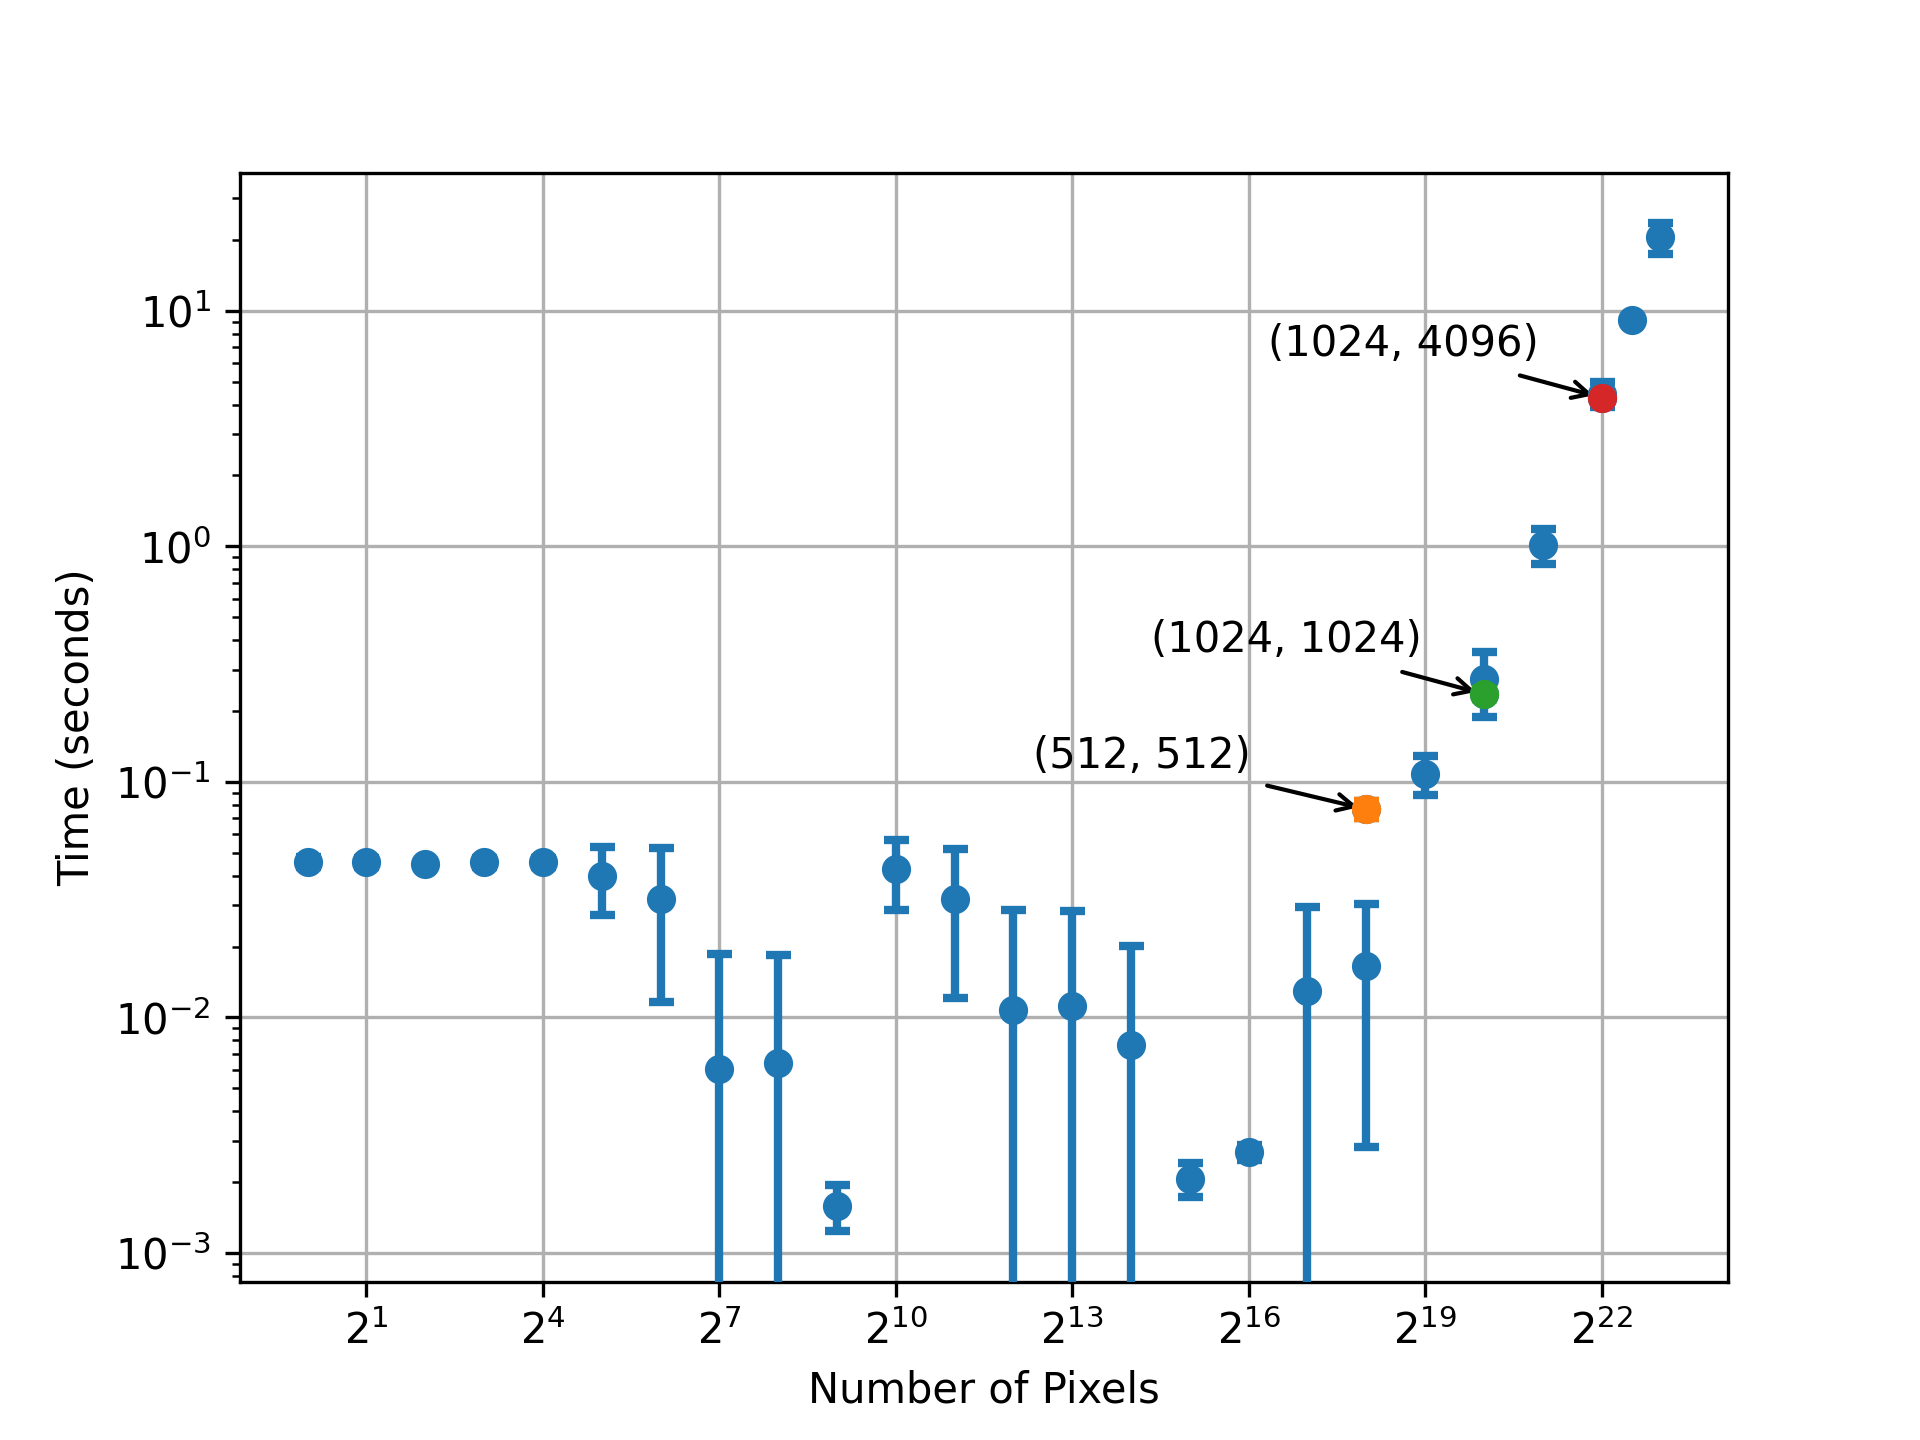
\includegraphics[width=.75\columnwidth]{figures/scaling/scaling}
	\caption{\label{si:fig:scaling} Scaling of transport time as a function of number of pixels for 32-bit integer arrays. Both the x- and y-axes are logarithmically scaled. Common camera sizes (512, 512), (1024, 1024), and (1024, 4096) are highlighted to provide context for camera users.}
\end{figure}

Common camera sizes (512, 512), (1024, 1024), and (1024, 4096) are highlighted in \ref{si:fig:scaling} to provide context.

There are some strategies that could be used to mitigate the performance problems of large cameras, but they have not been implemented because large arrays remain an edge case among current \yaq{} users.
Such strategies could include enabling compression, using transport layers other than TCP, using regions-of-interest (ROIs) to limit array sizes, and writing arrays locally to disk and providing mechanisms for retrieval out of band.
The Avro Specification \cite{AvroSpecification} specifically provides for compression codecs in the case of storing to disk, but there is nothing preventing the RPC pipe from similarly encoding the data, provided both ends of the communication support it.
This would allow larger arrays to be transported using fewer bytes over TCP, which would likely improve performance for large arrays where TCP transport is the bottleneck.
While TCP is the only currently supported transport layer for \yaq{}, this limitation could be lifted in the future.
TCP was chosen as the preferred starting point because it is ubiquitous, being available on every desired platform and implementation language.
One alternative that would be relatively easy to support would be Unix domain sockets (UDS).
UDS has an extremely similar interface to TCP sockets, and are handled in Python by the same standard library module.
UDS is potentially more performant, but as the name suggests are limited to Unix-like systems (i.e. it will not work on Windows).
ROIs are implemented on the handful of cameras currently in the \yaq{} ecosystem \cite{yaqd_andor,yaqd_pi}, however we are still in the experimentation phase and have not standardized ROI configuration into a \yaq{} trait.
When only a subset of the total camera area is interesting, this is one way to limit array size over the interface.
Finally \yaq{} daemons could be implemented to write arrays locally to disk, rather than transferring over the \yaq{} interface directly.
This has not yet been implemented, and would require clients to have knowledge of how to retrieve and display the images collected, but there is nothing preventing this if throughput is a limitation.
If such behavior became a standard feature desired for cameras, it should be encapsulated in a \yaq{} trait to provide a consistent interface.

To reproduce this figure, you will need the libraries specified in ``figures/requirements.txt''.
The scripts for generating this figure, including the \yaq{} daemon, are located in ``figures/scaling''.
To generate the data, run the \yaq{} daemon using \texttt{python scaling.py --config config.toml} from with in the ``scaling'' folder.
Then run \texttt{python scaling-data-gen.py}, which will communicate with the running daemon and produce a CSV written to standard out.
The result can be saved to \texttt{scaling.csv}.
To visualize the results, run \texttt{python plot-scaling.py}, which will read the CSV and produce the image.

\clearpage

\section{\texttt{yaqd-control}: tooling for managing \yaq{} daemons}

\texttt{yaqd-control} is a command line utility provided by the \yaq{} project to manage \yaq{} daemons.
The primary purpose of the tool is to maintain a list of active daemons, provide access to their configuration, and their running state.
This includes querying the active state of known daemons, as well as starting daemons running as backgound services.

\subsection{installation}

yaqd-control can be installed via
PyPI\cite{yaqd-control} or
conda-forge\cite{yaqd-control-conda}.

\begin{codefragment}{bash}
$ pip install yaqd-control
\end{codefragment}

\begin{codefragment}{bash}
$ conda config --add channels conda-forge
$ conda install yaqd-control
\end{codefragment}

\subsection{Usage}

yaqd-control is a command line application.

Help: learn more, right from your terminal.

\begin{codefragment}{bash}
$ yaqd --help
Usage: yaqd [OPTIONS] COMMAND [ARGS]...

Options:
  --help  Show this message and exit.

Commands:
  clear-cache
  disable
  edit-config
  enable
  list
  reload
  restart
  scan
  start
  status
  stop
\end{codefragment}

Try \texttt{yaqd\ \ -\/-help} to learn more about a particular command.

\paragraph{the cache}\label{the-cache}

yaqd-control keeps track of known daemons, referred to as the cache

Status: yaqd-control can quickly show you the status of all daemons in
yaqd-control's cache. This is usually the most used subcommand, as it
gives a quick overview of the system, which daemons are offline, and
which are currently busy.

\begin{codefragment}{bash}
$ yaqd status
+-----------+-------+--------------------------+------+---------+-------+
| host      | port  | kind                     | name | status  | busy  |
+-----------+-------+--------------------------+------+---------+-------+
| 127.0.0.1 | 38202 | system-monitor           | foo  | online  | False |
| 127.0.0.1 | 39054 | fake-continuous-hardware | bar  | online  | True  |
| 127.0.0.1 | 39055 | fake-continuous-hardware | baz  | online  | False |
| 127.0.0.1 | 39056 | fake-continuous-hardware | spam | offline | ?     |
| 127.0.0.1 | 37067 | fake-discrete-hardware   | ham  | online  | False |
| 127.0.0.1 | 37066 | fake-discrete-hardware   | eggs | online  | False |
+-----------+-------+--------------------------+------+---------+-------+
\end{codefragment}

List: this is essentially the same as \texttt{status} except that it
does not attempt to contact the daemons, so it does not give you
additional context. List supports a flag \texttt{--format} which accepts "json",
"toml", "prettytable", or "happi".

\begin{codefragment}{bash}
$ yaqd list
+-----------+-------+--------------------------+------+
| host      | port  | kind                     | name |
+-----------+-------+--------------------------+------+
| 127.0.0.1 | 38202 | system-monitor           | foo  |
| 127.0.0.1 | 39054 | fake-continuous-hardware | bar  |
| 127.0.0.1 | 39055 | fake-continuous-hardware | baz  |
| 127.0.0.1 | 39056 | fake-continuous-hardware | spam |
| 127.0.0.1 | 37067 | fake-discrete-hardware   | ham  |
| 127.0.0.1 | 37066 | fake-discrete-hardware   | eggs |
+-----------+-------+--------------------------+------+
\end{codefragment}

Scan: Scanning allows you to add currently running daemons to the cache.

\begin{codefragment}{bash}
$ yaqd scan
scanning host 127.0.0.1 from 36000 to 39999...
...saw unchanged daemon fake-discrete-hardware:eggs on port 37066
...saw unchanged daemon fake-discrete-hardware:ham on port 37067
...found new daemon system-monitor:foo on port 38202
...found new daemon fake-continuous-hardware:bar on port 39054
...saw unchanged daemon fake-continuous-hardware:baz on port 39055
...known daemon fake-continuous-hardware:spam on port 39056 not responding
...done!
\end{codefragment}

Scan has some additional options, passed as flags on the command line,
which allow you to change the default scan range and host (for remotely
accessed daemons):

\begin{codefragment}{bash}
$ yaqd scan --help
Usage: yaqd scan [OPTIONS]

Options:
  --host TEXT      Host to scan.
  --start INTEGER  Scan starting point.
  --stop INTEGER   Scan stopping point.
  --help           Show this message and exit.
\end{codefragment}

Edit Config: yaqd-control provides an easy way to edit the default
config file location for a daemon kind. This uses your default editor
(\texttt{EDITOR} environment variable), and defaults to \texttt{notepad.exe} on
Windows, and \texttt{vi} on other platforms. Using yaqd-control to edit
config files means that you do not need to know the default location.
Additionally, it does some basic validity checks (that the toml parses
and that each daemon section has the \texttt{port} keyword). If an error
is found, you are prompted to re-edit the file. Daemons from the config
file are added to the cache. You may pass multiple daemon kinds, which
will be opened in succession.

\begin{codefragment}{bash}
$ yaqd edit-config fake-continuous-hardware system-monitor
\end{codefragment}

Clear Cache: Note that this is a destructive action.
\texttt{clear-cache} deletes all daemons from the cache (thus
\texttt{list} and \texttt{status} will give empty tables) There is no
user feedback.

\begin{codefragment}{bash}
$ yaqd clear-cache
$ yaqd status
+------+------+------+------+--------+------+
| host | port | kind | name | status | busy |
+------+------+------+------+--------+------+
+------+------+------+------+--------+------+
\end{codefragment}

\paragraph{Running in the background}\label{running-in-the-background}
Each of the commands in this section can take multiple daemon kinds.
Enable: by enabling a daemon, you allow the operating system to manage
that daemon in the background. An enabled daemon will always start again
when you restart your computer. Enabling is required for the rest of the
commands in this section to work as expected. After enabling, it's
typical to start the daemon as well, this does not happen automatically.
Enablement works in slightly different ways on different platforms, but
the commands are the same (don't worry if the password prompts are
different). Currently supported platforms are Linux (systemd), MacOS
(launchd) and Windows (via NSSM, bundled with the distribution).

\begin{codefragment}{bash}
$ yaqd enable system-monitor
[sudo] password for scipy2020:
==== AUTHENTICATING FOR org.freedesktop.systemd1.manage-unit-files ===
Authentication is required to manage system service or unit files.
Password:
==== AUTHENTICATION COMPLETE ===
\end{codefragment}

Disable: this is the inverse operation to enable, which makes it so that
the daemon does not start on reboot. This does not affect the running
daemon.

\begin{codefragment}{bash}
$ yaqd disable system-monitor
==== AUTHENTICATING FOR org.freedesktop.systemd1.manage-unit-files ===
Authentication is required to manage system service or unit files.
Password:
==== AUTHENTICATION COMPLETE ===
Removed /etc/systemd/system/multi-user.target.wants/yaqd-system-monitor.service.
\end{codefragment}

Start: This starts the daemon running in the background immediately. It
must have been enabled to run in the background using this command.

\begin{codefragment}{bash}
$ yaqd start system-monitor
==== AUTHENTICATING FOR org.freedesktop.systemd1.manage-units ===
Authentication is required to start 'yaqd-system-monitor.service'.
Password:
==== AUTHENTICATION COMPLETE ===
\end{codefragment}

Stop: This stops the daemon running in the background immediately. It
must have been running in the background using yaqd-control (either on
startup via enable or via the start command above).

\begin{codefragment}{bash}
$ yaqd stop system-monitor
==== AUTHENTICATING FOR org.freedesktop.systemd1.manage-units ===
Authentication is required to stop 'yaqd-system-monitor.service'.
Password:
==== AUTHENTICATION COMPLETE ===
\end{codefragment}

Restart/Reload: This stops (if running) and restarts the daemon running
in the background immediately. Reload is slightly different in that it
signals to the daemon to reload its configuration rather than completely
restart, but effectively it is the same as restart (and is a pure alias
where such a signal is not supported). It must have been enabled to run
in the background using this command.

\begin{codefragment}{bash}
$ yaqd restart system-monitor
==== AUTHENTICATING FOR org.freedesktop.systemd1.manage-units ===
Authentication is required to restart 'yaqd-system-monitor.service'.
Password:
==== AUTHENTICATION COMPLETE ===
\end{codefragment}


\clearpage

\section{Package size analysis}

The raw data for package size analysis was collected using Tokei\cite{tokei}, a command line tool for analysing line lengths of source code.
It includes breaking down line length into ``code'', ``comments'', and ``blank'' lines.
The package size data was curated into \texttt{figures/lines\_histogram.txt}, which includes annotations as to the ``type'' and ``class'' for each file.
The ``type'' annotation is one of ``stub'' (meaning that the bulk of the implementation is in another file), ``normal'' (an individual daemon with the bulk of its implementation), ``protocol'' (an implementation the provides for multiple daemons, such as those referred to by ``stub''s, or ``serial'' (the implementation of a serial protocol rather than a full fledged daemon).
The ``class'' refers to the primary function of the daemon and is one of the following values: ``is-sensor'' for detectors, ``has-position'' for setable hardware, ``serial'' (identical to ``type'' annotation), and ``other'' for daemons which do not fit in the above categories.

The plotting script \texttt{figures/lines\_histogram.py} can be used to generate the figure from this text file.
The figure uses the ``code'' lines to generate a histogram of file sizes in the \yaq{} python implementations.
This is a measurable proxy for the amount of work that implementing an individual \yaq{} daemon entails, though of course cannot capture the work involved in learning the lower level interface.

\clearpage

\printbibliography

\end{document}
